%% Detector-independent interface block diagram (fig:e2e_interface), Section 3.12 intro.
%% Same colour code as autonomous_pipeline.tex: red = trained in this work (frozen at inference),
%% blue = external pre-trained detector (frozen), grey = deterministic (no learned parameters).
%% Build: pdflatex e2e_interface.tex; output copied to ../e2e_interface.pdf
\documentclass[10pt,tikz,border=4pt]{standalone}
\usepackage[T1]{fontenc}
\usepackage{mathptmx}
\usepackage{amsmath,amssymb}
\usetikzlibrary{positioning,arrows.meta,calc}

\begin{document}
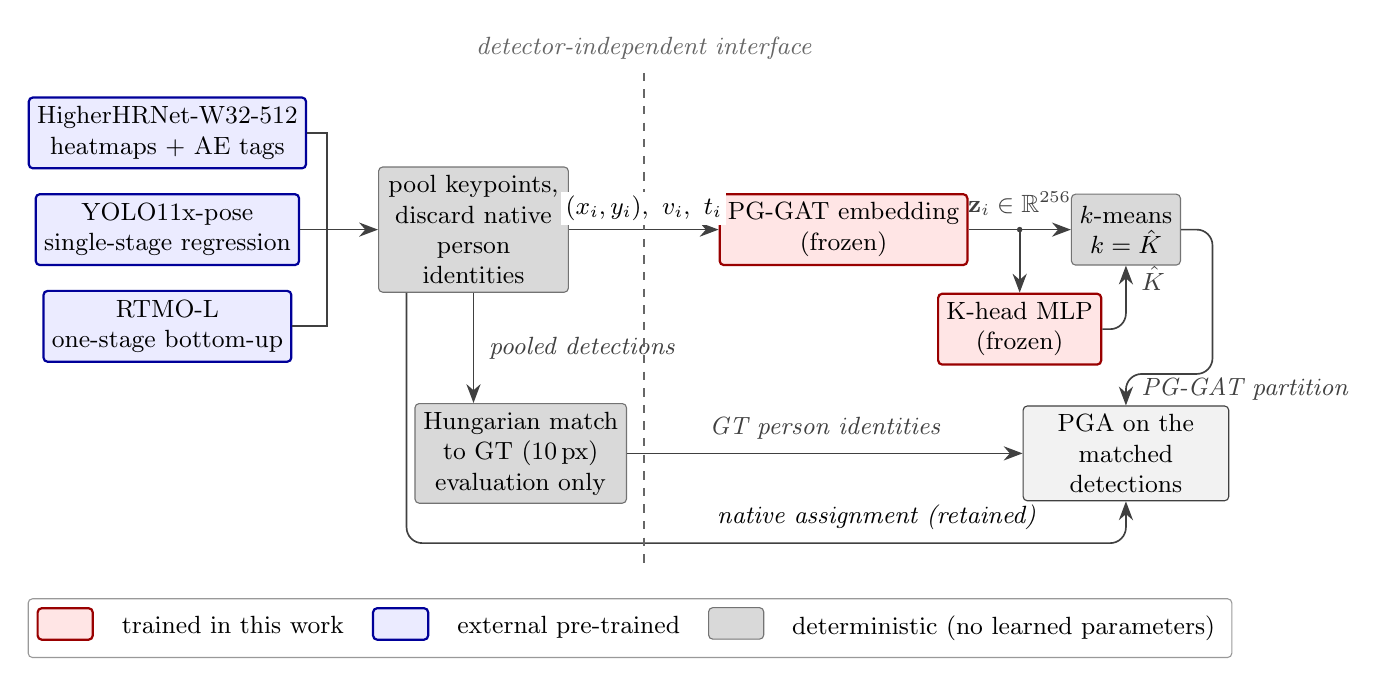
\begin{tikzpicture}[
  font=\small,
  >={Stealth[length=2.4mm]},
  box/.style={draw=black!75, rounded corners=1.5pt, align=center,
              inner sep=3pt, minimum height=9mm, fill=white},
  data/.style={box, fill=black!5},
  ours/.style={box, draw=red!60!black, fill=red!10, thick},
  ext/.style={box, draw=blue!60!black, fill=blue!8, thick},
  det/.style={box, draw=black!55, fill=black!15},
  arr/.style={->, semithick, black!75},
  line/.style={semithick, black!75},
  dlbl/.style={font=\small\itshape, align=center},
]

%% ---------- detectors (left column) ----------
\node[ext] (hr)   {HigherHRNet-W32-512\\ \textnormal{\small heatmaps $+$ AE tags}};
\node[ext, below=3mm of hr]   (yolo) {YOLO11x-pose\\ \textnormal{\small single-stage regression}};
\node[ext, below=3mm of yolo] (rtmo) {RTMO-L\\ \textnormal{\small one-stage bottom-up}};

%% ---------- pooling (native identities discarded) ----------
\coordinate (px) at ($(hr.east)+(9mm,0)$);
\node[det, text width=22mm, anchor=west] (pool) at (px |- yolo)
  {pool keypoints,\\ discard native\\ person identities};
%% one vertical bus, placed right of the widest detector box, collects the three detectors
\coordinate (bus) at ($(hr.east)+(2.5mm,0)$);
\coordinate (j) at ($(pool.west)+(-2.5mm,0)$);
\draw[line] (hr.east)   -- (bus |- hr.east)   -- (bus |- yolo.east);
\draw[line] (rtmo.east) -- (bus |- rtmo.east) -- (bus |- yolo.east);
\draw[line] (yolo.east) -- (j);
\draw[arr]  (j) -- (pool.west);

%% ---------- grouping module (right of the interface) ----------
\node[ours, right=19mm of pool] (pggat) {PG-GAT embedding\\ \textnormal{\small (frozen)}};
\node[det, right=13mm of pggat] (kmeans) {$k$-means\\ $k=\hat K$};
\coordinate (branch) at ($(pggat.east)!0.5!(kmeans.west)$);
\node[ours, below=8mm of branch, anchor=north] (khead) {K-head MLP\\ \textnormal{\small (frozen)}};

\draw[arr] (pool) -- (pggat);
\draw[arr] (pggat) -- node[dlbl, above=0.5mm]{$\mathbf{z}_i \in \mathbb{R}^{256}$} (kmeans);
\fill[black!75] (branch) circle (1pt);
\draw[arr] (branch) -- (khead.north);
\draw[arr, rounded corners=2mm] (khead.east) -| node[dlbl, pos=0.9, right=0.7mm]{$\hat K$} (kmeans.south);

%% ---------- evaluation row ----------
\node[det] (match) at ($(pool.south)+(6mm,-14mm)$) [anchor=north]
  {Hungarian match\\ to GT (10\,px)\\ \textnormal{\small evaluation only}};
\node[data, text width=24mm] (pga) at (kmeans.center |- match.center)
  {PGA on the matched\\ detections};

\draw[arr] (pool.south) -- node[dlbl, right=0.7mm]{pooled detections} (pool.south |- match.north);
\draw[arr] (match) -- node[dlbl, above=0.5mm]{GT person identities} (pga);
\draw[arr, rounded corners=2mm] (kmeans.east) -- ++(4mm,0) |- ($(pga.north)+(0,4mm)$) -- node[dlbl, pos=0.5, right=0.7mm]{PG-GAT partition} (pga.north);
%% native assignment: leaves the pooling box underside, left of the matching box, runs beneath it, enters PGA from below
\coordinate (nx) at ($(pool.south)+(-8.5mm,0)$);
\coordinate (n2) at ($(match.south)+(0,-5mm)$);
\draw[arr, rounded corners=2mm] (nx) -- (nx |- n2) -- (pga.center |- n2) -- (pga.south);
\node[dlbl, above=0.5mm] at ($(match.east |- n2)!0.5!(pga.center |- n2)$) {native assignment (retained)};

%% ---------- the interface ----------
\coordinate (ifx) at ($(pool.east)!0.5!(pggat.west)$);
\draw[dashed, thick, black!60] ($(ifx |- hr.north)+(0,3mm)$) -- ($(ifx |- n2)+(0,-3mm)$);
\node[dlbl, black!60, anchor=south] at ($(ifx |- hr.north)+(0,3.5mm)$) {detector-independent interface};

\node[dlbl, fill=white, inner sep=1.5pt, above=0.5mm] at ($(pool.east)!0.5!(pggat.west)$) {$(x_i, y_i),\ v_i,\ t_i$};

%% ---------- legend ----------
\matrix[draw=black!40, rounded corners=1.5pt, inner sep=3pt, column sep=2.5mm, row sep=1mm,
        ampersand replacement=\&] (leg)
        at ($(hr.west |- n2)+(0,-7mm)$) [anchor=north west] {
  \node[ours, minimum height=4mm, minimum width=7mm, inner sep=1pt] {}; \&
  \node[align=left]{trained in this work}; \&
  \node[ext, minimum height=4mm, minimum width=7mm, inner sep=1pt] {}; \&
  \node[align=left]{external pre-trained}; \&
  \node[det, minimum height=4mm, minimum width=7mm, inner sep=1pt] {}; \&
  \node[align=left]{deterministic (no learned parameters)}; \\
};

\end{tikzpicture}
\end{document}
